%%%%%%%%%%%%%%%%%%%%%%%%%%%%%%%%%%%%%%%%%%%%%%%%%%%%%%%%%%%%
%%  This Beamer template was created by Cameron Bracken.
%%  Anyone can freely use or modify it for any purpose
%%  without attribution.
%%
%%  Last Modified: January 9, 2009
%%

\documentclass[xcolor=x11names,compress]{beamer}


%% General document %%%%%%%%%%%%%%%%%%%%%%%%%%%%%%%%%%
\usepackage{graphicx}
\usepackage{tikz}
\usepackage[latin1]{inputenc}  
\usetikzlibrary{decorations.fractals}
%%%%%%%%%%%%%%%%%%%%%%%%%%%%%%%%%%%%%%%%%%%%%%%%%%%%%%


%% Beamer Layout %%%%%%%%%%%%%%%%%%%%%%%%%%%%%%%%%%
\beamertemplatenavigationsymbolsempty 
\useoutertheme[subsection=false,shadow]{miniframes}
  \setbeamertemplate{footline}%{miniframes theme}
  {%
    \begin{beamercolorbox}[colsep=1.0pt]{upper separation line foot}
    \end{beamercolorbox}
    \begin{beamercolorbox}[ht=0.25ex,dp=1.125ex,%
      leftskip=.3cm,rightskip=.3cm plus1fil]{author in head/foot}%
      \leavevmode{\usebeamerfont{author in head/foot}\insertshortauthor}%
      \hfill%
      {\usebeamerfont{institute in head/foot}\usebeamercolor[fg]{institute in head/foot}\insertshortinstitute}%
    \end{beamercolorbox}%
    \begin{beamercolorbox}[ht=2.5ex,dp=1.125ex,%
      leftskip=.3cm,rightskip=.3cm plus1fil]{title in head/foot}%
      {\usebeamerfont{title in head/foot}\insertshorttitle} \hfill     \Large{\insertframenumber}%
    \end{beamercolorbox}%
    \begin{beamercolorbox}[colsep=1.0pt]{lower separation line foot}
    \end{beamercolorbox}
  }

\useinnertheme{default}
%\usefonttheme{serif}
\usepackage{helvet}

\setbeamerfont{title like}{shape=\scshape}
\setbeamerfont{frametitle}{shape=\scshape}

\definecolor{playGreen}{RGB}{146,209,61}
\definecolor{textGrey}{RGB}{69,69,69}
\definecolor{backgroundColor}{RGB}{230,230,230}

\setbeamercolor*{lower separation line head}{bg=playGreen} 
\setbeamercolor*{normal text}{fg=textGrey,bg=backgroundColor} 
\setbeamercolor*{alerted text}{fg=red} 
\setbeamercolor*{example text}{fg=black} 
\setbeamercolor*{structure}{fg=black} 
 
\setbeamercolor*{palette tertiary}{fg=black,bg=black!10} 
\setbeamercolor*{palette quaternary}{fg=black,bg=black!10} 


\renewcommand{\(}{\begin{columns}}
\renewcommand{\)}{\end{columns}}
\newcommand{\<}[1]{\begin{column}{#1}}
\renewcommand{\>}{\end{column}}
%%%%%%%%%%%%%%%%%%%%%%%%%%%%%%%%%%%%%%%%%%%%%%%%%%

\setbeamertemplate{section page}
{
  \begin{centering}
    \vskip1em\par
    \begin{beamercolorbox}[sep=4pt,center]{part title}
      \usebeamerfont{section title}\insertsection\par
    \end{beamercolorbox}
  \end{centering}
}

\AtBeginSection[]
{
\frame{\sectionpage}
\begin{frame}<beamer>
\frametitle{Outline}
\tableofcontents[
  currentsection,
  sectionstyle=show/hide,
  subsectionstyle=show/show/hide
]
\end{frame}
}


\begin{document}


%%%%%%%%%%%%%%%%%%%%%%%%%%%%%%%%%%%%%%%%%%%%%%%%%%%%%%
%%%%%%%%%%%%%%%%%%%%%%%%%%%%%%%%%%%%%%%%%%%%%%%%%%%%%%
{
\setbeamercolor{background canvas}{bg=playGreen}
\setbeamercolor{title}{fg=white,bg=playGreen} 
\begin{frame}
\title{\textbf{Presentation patterns for web applications with Play! Framework}}
%\subtitle{SUBTITLE}
\author{
	Alberto Garc�a Garc�a\\
	{\it $<$ agg180@alu.ua.es $>$}\\
}
\date{
	
\includegraphics[height=30px]{play.png} %~ ~ 
\includegraphics[height=20px]{backbone.png}
	\\
	\vspace{1cm}
	\normalsize{\today}
}
\titlepage
\end{frame}
}

%%%%%%%%%%%%%%%%%%%%%%%%%%%%%%%%%%%%%%%%%%%%%%%%%%%%%%
%%%%%%%%%%%%%%%%%%%%%%%%%%%%%%%%%%%%%%%%%%%%%%%%%%%%%%

\begin{frame}{Table of Contents}
\tableofcontents[hideallsubsections]
\end{frame}

%%%%%%%%%%%%%%%%%%%%%%%%%%%%%%%%%%%%%%%%%%%%%%%%%%%%%%
%%%%%%%%%%%%%%%%%%%%%%%%%%%%%%%%%%%%%%%%%%%%%%%%%%%%%%

\section{\scshape Introduction}
\subsection{Trends}
\begin{frame}
\frametitle{Trends}
	\begin{itemize}
		\item{Enterprises's needs lead the market.}
		\item{Offering services: SOA wins.}
		\item{The web changes the status quo.}
		\item{SOA is not web compliant.}
		\item{Exposing services through the web requires extra effort.}
		\item{The game changes: new possibilities and challenges.}
	\end{itemize}
\end{frame}

%%%%%%%%%%%%%%%%%%%%%%%%%%%%%%%%%%%%%%%%%%%%%%%%%%%%%%
%%%%%%%%%%%%%%%%%%%%%%%%%%%%%%%%%%%%%%%%%%%%%%%%%%%%%%

\subsection{Challenges}
\begin{frame}
\frametitle{Challenges}
	\begin{itemize}
		\item{Real time data has to be pushed.}
		\item{Huge amounts of data.}
		\item{Need for scalability and integration.}
		\item{Easy integration and accessibility.}
		\item{Interoperability.}
	\end{itemize}
\end{frame}

%%%%%%%%%%%%%%%%%%%%%%%%%%%%%%%%%%%%%%%%%%%%%%%%%%%%%%
%%%%%%%%%%%%%%%%%%%%%%%%%%%%%%%%%%%%%%%%%%%%%%%%%%%%%%

\subsection{Addressing the challenges}
\begin{frame}
\frametitle{Addressing the challenges}
	\begin{itemize}
		\item{Embrace the internet.}
		\begin{itemize}
			\item{HTTP Protocol}
			\item{HTML5}
			\item{XML/JSON}
			\item{Javascript}
			\item{CSS}
		\end{itemize}
		\item{Paradigm shift: client-side.}
		\item{Simplicity.}
		\item{A framework to rule them all.}
		\item{\Large{\textbf{Patterns for enterprise applications}.}}
	\end{itemize}
\end{frame}

%%%%%%%%%%%%%%%%%%%%%%%%%%%%%%%%%%%%%%%%%%%%%%%%%%%%%%
%%%%%%%%%%%%%%%%%%%%%%%%%%%%%%%%%%%%%%%%%%%%%%%%%%%%%%

\section{\scshape Play! Framework}
\subsection{What is Play! Framework?}
\begin{frame}{What is Play! Framework?}
	\begin{itemize}
		\item{A web framework focused on:}
		\begin{itemize}
			\item{Simplicity.}
			\item{Productivity.}
			\item{Scalability.}
			\item{Designed for the modern web.}
			\begin{itemize}
				\item{Concentrate on server-side.}
				\item{Delegate AMAP to the client.}
			\end{itemize}
			\item{Embrace internet standards.}
			\item{Java and Scala.}
			\item{RESTful architecture web applications.}
			\item{Model-View-Controller.}
		\end{itemize}
	\end{itemize}
\end{frame}

%%%%%%%%%%%%%%%%%%%%%%%%%%%%%%%%%%%%%%%%%%%%%%%%%%%%%%
%%%%%%%%%%%%%%%%%%%%%%%%%%%%%%%%%%%%%%%%%%%%%%%%%%%%%%

\subsection{RESTful Architecture}
\begin{frame}{RESTful architecture}
	\begin{itemize}
		\item{Implemented using HTTP and REST principles.}
		\item{Representational state transfer (REST) principles:}
		\begin{itemize}
			\item{Uniform interface.}
			\item{Stateless.}
			\item{Caching.}
			\item{Layers.}
			\item{Code on demand.}
		\end{itemize}
		\item{Goals:}
		\begin{itemize}
			\item{Performance.}
			\item{Scalability.}
			\item{Portability.}
			\item{Reliability.}
			\item{SIMPLICITY.}
		\end{itemize}
	\end{itemize}
\end{frame}

%%%%%%%%%%%%%%%%%%%%%%%%%%%%%%%%%%%%%%%%%%%%%%%%%%%%%%
%%%%%%%%%%%%%%%%%%%%%%%%%%%%%%%%%%%%%%%%%%%%%%%%%%%%%%

\subsection{Project layout}
\begin{frame}{Project layout}
	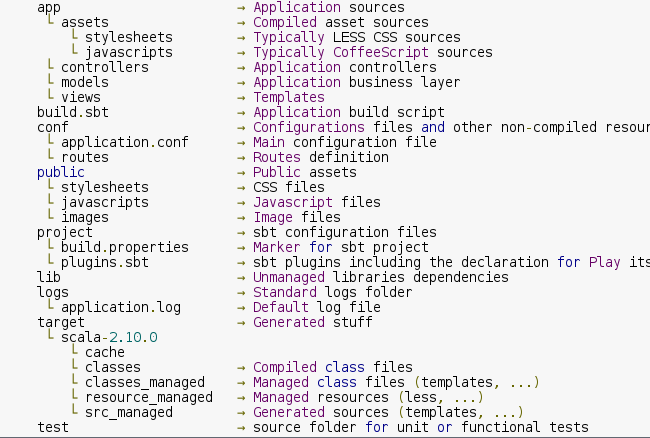
\includegraphics[height=200px]{layout.png}
\end{frame}


%%%%%%%%%%%%%%%%%%%%%%%%%%%%%%%%%%%%%%%%%%%%%%%%%%%%%%
%%%%%%%%%%%%%%%%%%%%%%%%%%%%%%%%%%%%%%%%%%%%%%%%%%%%%%

\section{\scshape Patterns in Play!}
\begin{frame}{Patterns in Play!}
	\begin{itemize}
		\item{\textbf{Model-View-Controller}.}
		\item{Model.}
		\begin{itemize}
			\item{Object-Relational Mapping.}
		\end{itemize}
		\item{Controller.}
		\begin{itemize}
			\item{Front Controller.}
		\end{itemize}
		\item{View.}
		\begin{itemize}
			\item{Template View.}
			\item{Composite View.}
		\end{itemize}
	\end{itemize}
\end{frame}

%%%%%%%%%%%%%%%%%%%%%%%%%%%%%%%%%%%%%%%%%%%%%%%%%%%%%%
%%%%%%%%%%%%%%%%%%%%%%%%%%%%%%%%%%%%%%%%%%%%%%%%%%%%%%

\subsection{Model-View-Controller}
\subsubsection{The MVC application model}
\begin{frame}{The MVC application model}
	\begin{itemize}
		\item{Models in app/models}
		\begin{itemize}
			\item{Java/Scala classes.}
			\item{Data + Operations, mainly object-oriented.}
			\item{Business logic and storage.}
		\end{itemize}
		\item{Views in app/views}
		\begin{itemize}
			\item{HTML/XML/JSON/Scala templates.}
			\item{Directives as placeholders for data.}
			\item{Render models to user interfaces.}
		\end{itemize}
		\item{Controllers in app/controllers}
		\begin{itemize}
			\item{Java/Scala classes.}
			\item{Methods as actions, mainly procedural.}
			\item{Receive requests, act (update models + render views) and response.}
		\end{itemize}
	\end{itemize}
\end{frame}

%%%%%%%%%%%%%%%%%%%%%%%%%%%%%%%%%%%%%%%%%%%%%%%%%%%%%%
%%%%%%%%%%%%%%%%%%%%%%%%%%%%%%%%%%%%%%%%%%%%%%%%%%%%%%

\subsubsection{Request/Response path}
\begin{frame}{Request/Response flow}
	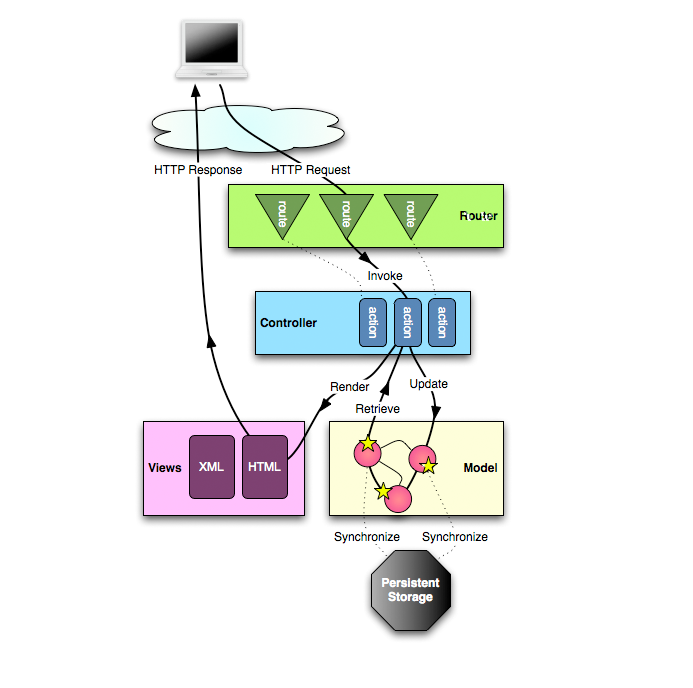
\includegraphics[height=200px]{diagrams_path.png}
\end{frame}

%%%%%%%%%%%%%%%%%%%%%%%%%%%%%%%%%%%%%%%%%%%%%%%%%%%%%%
%%%%%%%%%%%%%%%%%%%%%%%%%%%%%%%%%%%%%%%%%%%%%%%%%%%%%%

\subsection{Model}
\subsubsection{Object Relational Mapping}
\begin{frame}{Object Relational Mapping}
	\begin{itemize}
		\item{a}
	\end{itemize}
\end{frame}

%%%%%%%%%%%%%%%%%%%%%%%%%%%%%%%%%%%%%%%%%%%%%%%%%%%%%%
%%%%%%%%%%%%%%%%%%%%%%%%%%%%%%%%%%%%%%%%%%%%%%%%%%%%%%

\subsection{View}
\subsubsection{Template View}
\begin{frame}{Template View}
	\begin{itemize}
		\item{\begin{quote}
		"Renders information into HTML by embedding markers in an HTML page"\cite{PEAA}
		\end{quote}}
	\end{itemize}
	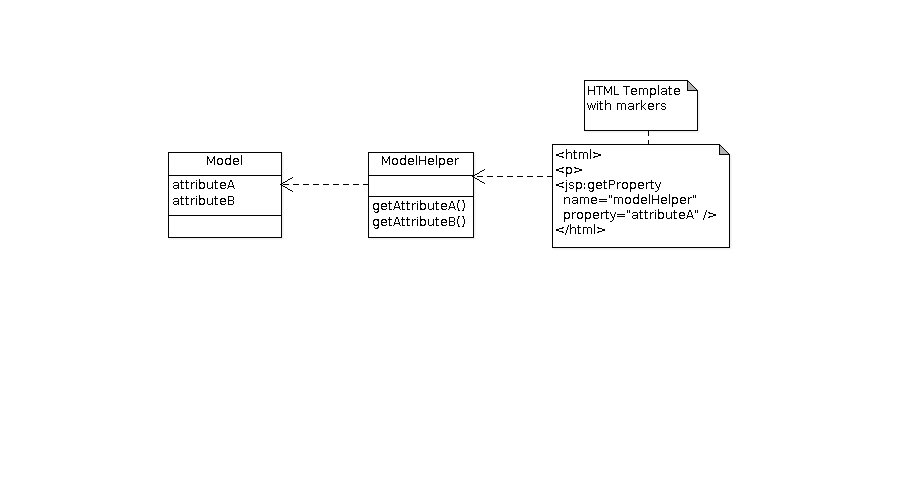
\includegraphics[clip=true,trim={120px 220px 100px 65px},height=110px]{templateview.png}
			\begin{itemize}
				\item{Pros: Centralized control, Thread safety, Configurability.}
				\item{Cons: Possible performance issues, Maintenance costs.}
			\end{itemize}
\end{frame}

\begin{frame}{Template View}
	\begin{itemize}
		\item{\begin{quote}
		The template with annotations is compiled to a Scala.class with a render() method with the template parameters.
		\end{quote}}
	\end{itemize}
	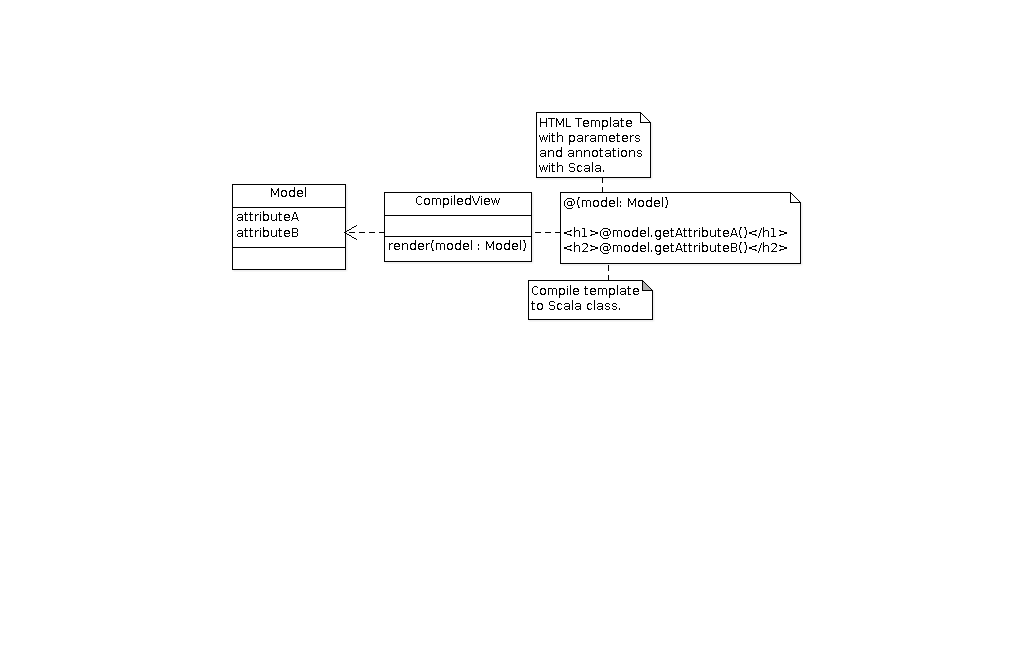
\includegraphics[clip=true,trim={200px 350px 100px 110px},height=110px]{templateviewplay.png}
			\begin{itemize}
				\item{The controller calls the render method of the view.}
				\item{The view communicates with the model (parameter).}
			\end{itemize}
\end{frame}

%%%%%%%%%%%%%%%%%%%%%%%%%%%%%%%%%%%%%%%%%%%%%%%%%%%%%%
%%%%%%%%%%%%%%%%%%%%%%%%%%%%%%%%%%%%%%%%%%%%%%%%%%%%%%

\subsubsection{Composite View}
\begin{frame}{Composite View}
	\begin{itemize}
		\item{a}
	\end{itemize}
\end{frame}

%%%%%%%%%%%%%%%%%%%%%%%%%%%%%%%%%%%%%%%%%%%%%%%%%%%%%%
%%%%%%%%%%%%%%%%%%%%%%%%%%%%%%%%%%%%%%%%%%%%%%%%%%%%%%

\subsection{Controller}
\subsubsection{Front Controller}
\begin{frame}{Front Controller Pattern}
	\begin{itemize}
		\item{\begin{quote}
		"Consolidates all request handling by channeling requests through a single handler object" \cite{PEAA}
		\end{quote}}
	\end{itemize}
	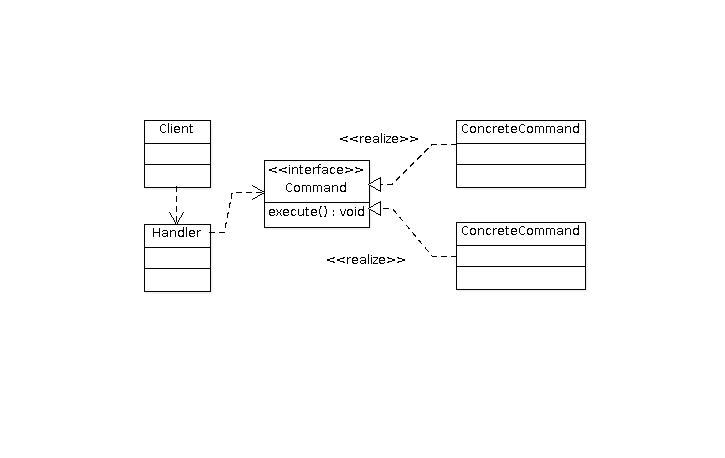
\includegraphics[clip=true,trim={50px 160px 100px 120px},height=90px]{frontcontroller.png}
		\begin{itemize}
			\item{Pros: Centralized control, Thread safety, Configurability.}
			\item{Cons: Possible performance issues, Maintenance costs.}
		\end{itemize}
\end{frame}

\begin{frame}{Front Controller in Play!}
	\begin{itemize}
		\item{The router (handler) selects a controller (command) and a particular action (execute) depeding on the HTTP request.}
	\end{itemize}
	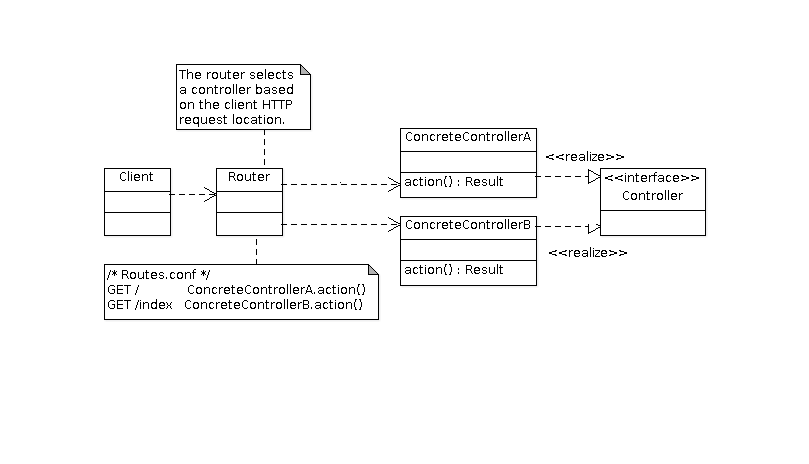
\includegraphics[clip=true,trim={50px 130px 100px 65px},height=120px]{frontcontrollerplay.png}
		\begin{itemize}
			\item{Routes.conf file determines the location-action relationship.}
			\item{Actions return a result that holds the HTTP Response.}
		\end{itemize}
\end{frame}

%%%%%%%%%%%%%%%%%%%%%%%%%%%%%%%%%%%%%%%%%%%%%%%%%%%%%%
%%%%%%%%%%%%%%%%%%%%%%%%%%%%%%%%%%%%%%%%%%%%%%%%%%%%%%

\section{\scshape Conclusions}
\begin{frame}
	\begin{itemize}
		\item{a}
	\end{itemize}
\end{frame}

%%%%%%%%%%%%%%%%%%%%%%%%%%%%%%%%%%%%%%%%%%%%%%%%%%%%%%
%%%%%%%%%%%%%%%%%%%%%%%%%%%%%%%%%%%%%%%%%%%%%%%%%%%%%%

\section*{\scshape References}
\begin{frame}
	\normalsize
	\nocite{PlayForJava}
	\nocite{PlayForScala}
	\nocite{PlayFrameworkCookbook}
	\frametitle{References}
	\bibliographystyle{amsalpha}
	\bibliography{biblio}
\end{frame}

\end{document}